\subsection{Locally Linear Embedding (LLE)}
\subsubsection{Tổng quan}

Locally Linear Embedding (LLE) là một thuật toán học không giám sát (Unsupervised Learning) dùng để giảm chiều dữ liệu phi tuyến thuộc nhóm \textit{Manifold}.

\begin{figure}[H]
	\begin{center}
		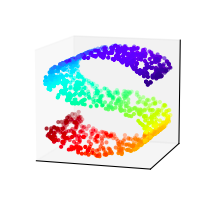
\includegraphics[scale=0.7]{images/ex1/manifold.png}
		\caption{Manifold}
	\end{center}
\end{figure}


Giải thuật LLE được nhóm tác giả \textit{Sam T. Roweis} và \textit{Lawrence K. Saul} trình bày trong bài báo "Nonlinear Dimensionality Reduction by Locally Linear Embedding" vào năm 2000.

\subsubsection{Các bài toán liên quan}
\begin{enumerate}
	\item \textbf{Face Recognition with Weighted Locally Linear Embedding}.\\ Bài toán nhận dạng khuôn mặt kết hợp với giảm chiều dữ liệu bằng thuật LLE. Qua các thực nghiệm, người ta có thể thấy rằng không gian các ảnh khuôn mặt là không gian phi tuyến có dạng đa tạp. Do đó, thuật toán LLE với khả năng giảm chiều dữ liệu phi tuyến của mình, có thể cho ra kết quả phân lớp tốt hơn so với sử dụng các giải thuật giải chiều kinh điển như PCA.
	\begin{figure}[H]
		\begin{center}
			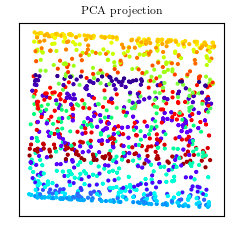
\includegraphics[scale=0.6]{images/ex1/pca.png}
			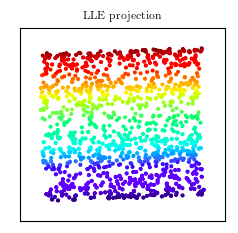
\includegraphics[scale=0.6]{images/ex1/lle.png}
			\caption{So sánh giảm chiều sử dụng PCA và LLE trên manifold}
		\end{center}
	\end{figure}
	\item \textbf{Audio Fingerprint Extraction Based on Locally LinearEmbedding for Audio Retrieval System}. 
	
	Bài toán so sánh giọng nói của một người với dữ liệu giọng nói trong database. Vấn đề của bài toán là dữ liệu âm thanh cần lưu trữ quá lớn và ảnh hưởng đến tốt độ chạy của hệ thống. Do đó, cần phải sử dụng thuật giảm chiều LLE để có thể biểu diễn âm thanh nhận dạng tốt hơn trong tập dữ liệu, giúp giảm bớt không gian lưu trữ và thời gian chạy được cải thiện.
	\begin{figure}[H]
		\begin{center}
			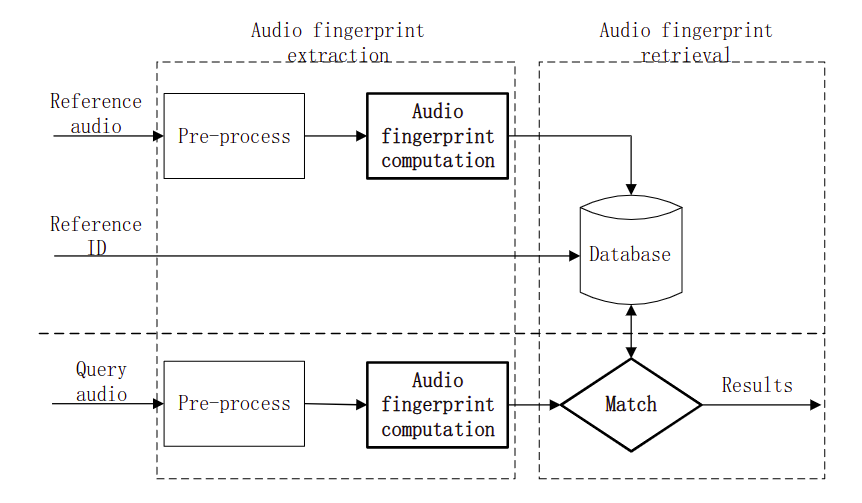
\includegraphics[scale=0.4]{images/ex1/audio-fingerprint}
			\caption{Hệ thống nhận dạng giọng nói}
		\end{center}
	\end{figure}
	\item \textbf{Supervised Locally Linear Embedding Algorithm for Hand Writting Recognition}.
	Bài toán nhận dạng chữ viết tay nói riêng và các bài toán nhận dạng mẫu nói chung thường gặp khó khăn khi chiều của dữ liệu tăng lên. Nhất là khi lượng dữ liệu trong tập không nhiều trong bài toán nhận dạng chữ viết tay. Chiều dữ liệu lớn làm cho việc nhận dạng trở nên khó khăn và tốn nhiều thời gian. Vì lý do đó, ta có thể sử dụng các thuật toán giảm chiều. 
	
	Bài toán sử dụng một một biến thể của LLE là \textit{Supervised LLE} (SLLE) để có thể áp dụng trên bài toán học có giám sát. Nhờ vào giảm chiều, sẽ tránh được các vấn đề về thiếu dữ liệu và chiều không gian lớn gây ảnh hưởng đến tính hiểu quả của giải thuật.
	\begin{figure}[H]
		\begin{center}
			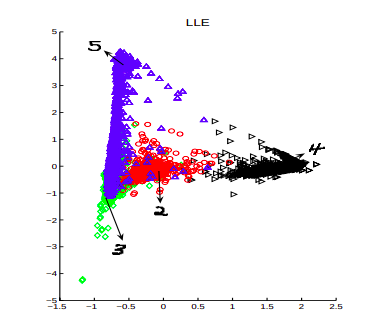
\includegraphics[scale=0.5]{images/ex1/MLLE.png}
			\caption{Hand writting Manifold}
		\end{center}
	\end{figure}
\end{enumerate}

\subsubsection{Mô tả thuật toán LLE}
\begin{enumerate}
	\item Với mỗi điểm dữ liệu p chiều, ta tìm k láng giềng gần nhất của nó.
	\item Tìm ma trận W sao cho tổng bình phương lỗi khi tái cấu trúc tuyến tính mỗi $x_i$ đạt giá trị nhỏ nhất:
	\begin{equation}
		\varepsilon(W) = \sum_{i=1}^{m}{\epsilon_i} = \sum_{i=1}^{m}{\left\|x_i - \sum_{j=1}^{n}{w_{ij}x_j}\right\|}
	\end{equation}
	\item Tìm Y sao cho tổng bình phương độ lỗi của quá trình tái cấu trúc đạt đạt giá trị nhỏ nhất:
	\begin{equation}
		\Theta(Y) = \sum_{i=1}^{n}{\left\|y_i - \sum_{j=1}^{n}{w_{ij}y_j}\right\|}
	\end{equation}
\end{enumerate}
\subsubsection{Đánh giá giải thuật}
\begin{itemize}
	\item \textbf{Ưu điểm}
	\begin{itemize}
		\item \textit{Siêu tham số}: Chỉ cần gán trước 2 siêu tham số.
		\item \textit{Tối ưu}: không liên quan đến cực tiểu cục bộ.
		\item \textit{Bảo toàn thông tin}: Thông tin không gian cục bộ trong không gian nhiều chiều được bảo toàn trong không gian con.
		\item \textit{Độ phức tạp:} LLE được cài đặt trong bộ thư viện scikit-learn là: $$\mathbf{O}[D log(k) m log(m)] + \mathbf{O}[Dmk^3] + \mathbf{0}[dm^2]$$
		Có thể thấy thuật toán chạy trong thời gian đa thức và phụ thuộc mạnh mẽ vào số lượng láng giếng k.
		\item \textit{Thư viện hỗ trợ:} Trong python, Locally Linear Embedding được cài đặt trong thư viện scikit-learn (sklearn.manifold.LocaLinearEmbedding).
	\end{itemize}
	\item \textbf{Nhược điểm}
	\begin{itemize}
		\item Nếu mật độ các mẫu không dày, hoặc việc lấy mẫu không đều, có thể tạo ra các manifold không đồng nhất, hay nói cách khác có nhiều manifold hình thành nên bộ dữ liệu, từ đó gây ra hiểu nhầm trong lúc chạy thuật.
		\item LLE rất nhạy cảm với nhiễu, với một lượng nhiễu nhỏ cũng có thể dẫn đên lỗi khi tạo embedding. 
		\item Không đảm bảo 2 điểm khác nhau trong không gian nhiều chiều sẽ khác nhau trong không gian giảm chiều. 
		\item Phụ thuộc nhiều vào 2 siêu tham số k và d. Việc chọn 2 siêu tham số không tốt có thể dẫn đến thuật toán không cho kết quả tốt.
		\item Chỉ dùng cho các bài toán học không giám sát. (Sau đó đã có các biến thể SLLE để giải quyết các bài toán học có giám sát).
	\end{itemize}
\end{itemize}